\documentclass[tikz]{standalone}
\usepackage{tikz}
\usepackage{siunitx}
\DeclareSIUnit\degF{\text{°}F}

\definecolor{codeblue}{RGB}{69, 161, 248}
\definecolor{codegray}{RGB}{40, 40, 40}
\usetikzlibrary{shapes,arrows}
\tikzstyle{decision} = [diamond, draw, fill=codegray, text=white,
    text width=4.5em, text badly centered, node distance=3cm, inner sep=0pt]
\tikzstyle{block} = [rectangle, draw, fill=codeblue,  text=white,
    text width=5em, text centered, rounded corners, minimum height=4em]
\tikzstyle{line} = [draw, -latex']


\begin{document}
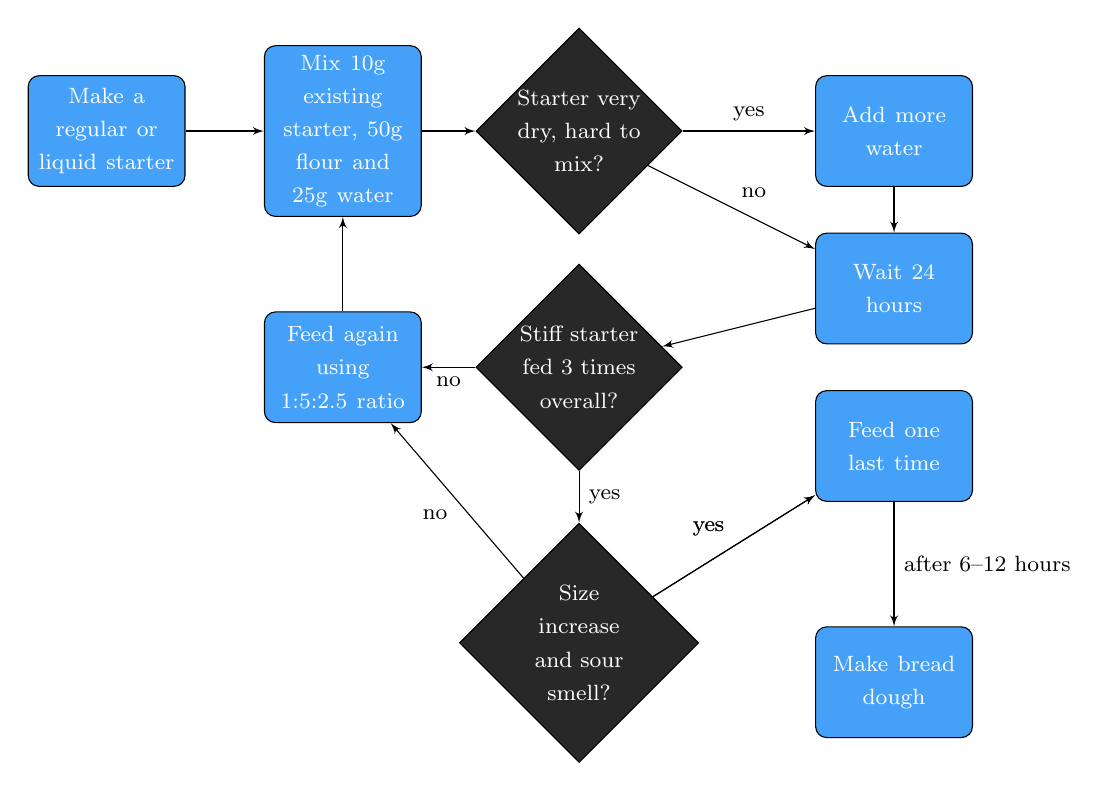
\begin{tikzpicture}[node distance = 3cm, auto]
  \node [block] (init) {\footnotesize Make a regular or liquid starter};
  \node [block, right of=init] (feed_new_ratio) {\footnotesize Mix 10g existing starter, 50g flour and 25g water};
  \node [decision, right of=feed_new_ratio, node distance=3cm] (too_dry) {\footnotesize Starter very dry, hard to mix?};
  \node [block, right of=too_dry, node distance=4cm] (add_water) {\footnotesize Add more water};
  \node [block, below of=add_water, node distance=2cm] (next_day) {\footnotesize Wait 24 hours};
  \node [decision, below of=too_dry, node distance=3cm] (repeated_3_times) {\footnotesize Stiff starter fed 3 times overall?};
  \node [block, left of=repeated_3_times] (feed_again) {\footnotesize Feed again using 1:5:2.5 ratio};
  \node [decision, below of=repeated_3_times, node distance=3.5cm] (ready_signs) {\footnotesize Size increase and sour smell?};
  \node [block, below of=next_day, node distance=2cm] (last_feed) {\footnotesize Feed one last time};
  \node [block, below of=last_feed, node distance=3cm] (bread_dough) {\footnotesize Make bread dough};
  \path [line] (init) -- (feed_new_ratio);
  \path [line] (feed_again) -- (feed_new_ratio);
  \path [line] (next_day) -- (repeated_3_times);
  \path [line] (repeated_3_times) -- node{\footnotesize yes} (ready_signs);
  \path [line] (repeated_3_times) -- node{\footnotesize no} (feed_again);
  \path [line] (ready_signs) -- node{\footnotesize no} (feed_again);
  \path [line] (ready_signs) -- node{\footnotesize yes} (last_feed);
  \path [line] (last_feed) -- node{\footnotesize after 6--12 hours} (bread_dough);
  \path [line] (feed_new_ratio) -- (too_dry);
  \path [line] (add_water) -- (next_day);
  \path [line] (too_dry) -- node{\footnotesize no} (next_day);
  \path [line] (too_dry) -- node{\footnotesize yes} (add_water);
  \path [line] (ready_signs) -- node{\footnotesize yes} (last_feed);
\end{tikzpicture}
\end{document}
